%\section{Tomy Prawoto}
%\subsection{Soal 1}
%Isi jawaban soal ke-1

%Kalau mau dibikin paragrap \textbf{cukup enter aja}, tidak usah pakai \verb|par| dsb

%\subsection{Soal 2}
%Isi jawaban soal ke-2

%\subsection{Soal 3}
%Isi jawaban soal ke-3

%%%%%%%%%%%%%%%%%%%%%%%%%%%%%%%%%%%%%%%%%%%%%%%%%%%%%%%%%%%%%%%%%%%%%%%%%%%%%%%%%%%%%%%%%%%%%%%%%%%

\section{Kaka Kamaludin}
\subsection{Soal 1}
folder /dev pada linux beriisi file konfigurasi hardware.
Device Manager berfungsi untuk mengatur driver hardware.

\subsection{Soal 2}
\begin{itemize}
	\item download Arduino Software(IDE)  
		https://www.arduino.cc/en/Main/Software
		download untuk linux
	\item extract file yang di download dan masuk ke folder hasil extract
	\item jalankan "./install.sh"
\end{itemize}

\subsection{Soal 3}
. . .

\subsection{Soal 4}
modul pyserial berfungsi untuk merangkum akses untuk port serial. moduk ini dapat di gunakan untuk python yang berjalan pada windows, osx, BSD (yang mendukung system POSIX) dan IronPython.Ini dirilis di bawah lisensi perangkat lunak gratis.

\subsection{Soal 5}
\begin{itemize}
	\item serial.Serial('/dev/tty*')
	membuka port serial
	
	\item ser.close()
	menutup port serial
	
	\item ser.read()
	membaca satu bit
	
	\item ser.readline()
	membaca line semua line
		
\end{itemize}

\subsection{Soal 6}
fungsi perulangan dibutuhkan untuk penggunaan code membutuhkan penggunaan contoh nya seperti multiple choce yang menggunakan perulangan tak terhingga 'while'.

\subsection{Soal 7}
\lstinputlisting[firstline=1, lastline=9]{src/5/1174067/Teori/1174067.py}

%%%%%%%%%%%%%%%%%%%%%%%%%%%%%%%%%%%%%%%%%%%%%%%%%%%%%%%%%%%%%%%%%%%%%%%%%%%%%%%%%%%%%%

\section{Ainul Filiani}
\begin{enumerate}
\item Apa itu fungsi device manager di windows dan folder /dev linux ?

Device Manager pada komputer Windows atau linux, diambil dari Microsoft Management Console. Pengelola Perangkat Menampilkan semua perangkat keras yang dapat diinisialisasi (dikenali) oleh Windows atau linux. Penampilan telah diatur (dikelompokkan) sehingga akan memudahkan pengelolaan setiap perangkat keras yang ada.
Pengelola Perangkat Windows atau linux
Device Manager akan sangat membantu dalam mengelola (mengelola) semua perangkat keras yang diinstal (dan diinstal) dalam sistem Windows atau linux. Perangkat keras seperti hard drive, kartu VGA, suara, keyboard, perangkat USB dll. Akan sangat mudah untuk mengaksesnya dari dalam Device Manager.

Beberapa fungsi kegunaan Manajer Perangkat meliputi:
\begin{enumerate}
\item Membahas status perangkat perangkat keras
\item Diskusikan informasi terperinci tentang perangkat keras
\item Kelola driver perangkat keras
\item Nonaktifkan dan Aktifkan perangkat keras
\item Mengatasi konflik perangkat keras, dll.
\end{enumerate}

\item Jelaskan Langkah-Langkah Instalasi Driver Dari Arduino ?

\begin{enumerate}
\item Menginstal Arduino IDE pada perangkat Windows: 

Karena file IDE Arduino yang dipilih dalam unduhan sebelumnya adalah format file .zip, file ini tidak memerlukan instalasi untuk digunakan, dengan kata lain, ini adalah file IDE Arduino yang portabel.
\item Pertama, silakan sambungkan Arduino ke PC Windows 10 atau laptop Anda menggunakan kabel USB
\item Setelah itu, buka Device Manager. Caranya adalah dengan hanya menekan tombol Windows + Pause Break secara bersamaan, lalu pilih Device Manager di menu sebelah kiri
\item Ketika Anda telah memasuki tampilan Device Manager, silakan pilih Ports (COM dan LPT). Setelah dipilih akan muncul drop down yang bertuliskan USB Serial Device (COM4)
\item Klik kanan pada bagian USB Serial Device (COM4), lalu pilih Update Driver
\item Setelah dua pilihan muncul, silakan pilih Browse my computer for software driver
\item Langkah selanjutnya silakan cari di mana folder Anda menyimpan driver Arduino. Karena itu, pastikan Anda memiliki driver. Jika Anda tidak memilikinya, silakan unduh terlebih dahulu
\item Setelah Anda memilih folder lokasi driver Arduino, silakan klik OK dan tunggu sampai proses instalasi driver selesai
\item Jika proses instalasi selesai dan berhasil, maka penulisan USB Serial Device (COM4) di Device Manager akan berubah menjadi Arduino Uno (COM4) atau seri lain sesuai dengan Arduino yang Anda gunakan
\item terakir Anda bisa langsung memasukkan program ke Arduino dari komputer

\end{enumerate}
\item Jelaskan bagaimana cara membaca baudrate dan port dari komputer yang sudah terinstall driver ? 

Untuk membaca baudrate bisa dicek melalui arduino IDE, setelah itu  untuk mengecheck port dapat dilakukan dengan device manager


\item Jelaskan sejarah library pyserial ? 

Modul ini merangkum akses untuk port serial. Ini menyediakan backends untuk Python yang berjalan di Windows, Linux, BSD (mungkin sistem yang mendukung POSIX), Jython dan IronPython (.NET dan Mono). Modul bernama "serial" secara otomatis memilih backend yang sesuai. Antarmuka berbasis kelas yang sama pada semua platform yang didukung.
Akses ke pengaturan port melalui properti Python.
Dukungan untuk berbagai ukuran byte, bit stop, paritas dan kontrol aliran dengan RTS / CTS dan / atau Xon / Xoff.
Bekerja dengan atau tanpa menerima batas waktu.
File seperti API dengan "read" dan "write" ("readline" dll. Juga didukung).
File-file dalam paket ini adalah 100 persen Python murni.
Port diatur untuk transmisi biner. Tidak ada stripping byte NULL, terjemahan CR-LF dll. (Yang berkali-kali diaktifkan untuk POSIX.) Ini membuat modul ini bermanfaat secara universal.
Kompatibel dengan pustaka io (Python 2.6+)

\item Jelaskan fungsi apa saja yang dipakai library pyserial ?
\begin{enumerate}
\item ‘A’	RELAY ON
\item ‘Z’	RELAY OFF
\item ‘1’	RELAY ON selama 100ms
\item ‘2’	RELAY ON selama 250ms
\item ‘3’	RELAY ON selama 500ms


\end{enumerate}
\item Jelaskan kenapa perlu pengulangan dalam tidak butuh perulangan dalam membaca serial ? 

Perualangan dalam bahasa pemrograman berfungsi menyuruh komputer melakukan sesuatu secara berulang-ulang. Terdapat dua jenis perualangan dalam bahasa pemrograman python, yaitu perulangan dengan for dan while.
Perulangan for disebut counted loop (perulangan yang terhitung), sementara perulangan while disebut uncounted loop (perulangan yang tak terhitung). Perbedaannya adalah perulangan for biasanya digunakan untuk mengulangi kode yang sudah diketahui banyak perulangannya. Sementara while untuk perulangan yang memiliki syarat dan tidak tentu berapa banyak perulangannya.
Perulangan diperlukan agar dapat membaca data secara berulang kali sehingga data yang muncul lebih dari satu.  Sedangkan apabila tidak memakai perulangan maka data akan terbaca satu kali saja.
\item Jelaskan cara membuat fungsi yang menggunakan pyserial ? 

Sebelum dapat menggunakan fungsi-fungsi PySerial dalam program, kita harus meng-import-nya terlebih dahulu dengan perintah:
import serial
Setelah itu  kita bisa mem-binding object SER2REL dengan port serial COM1 pada baudrate 2400.
SER2REL = serial.Serial(“COM1”, 2400)
Apabila  binding berhasil maka port serial COM1 akan di-open dan siap digunakan. Untuk mengetes apakah COM1 sudah open dan siap digunakan, kita gunakan fungsi isOpen sebagai berikut:
SER2REL.isOpen()
Fungsi ini menghasilkan nilai True jika COM1 sudah open dan nilai False jika sebaliknya. Pada eksperimen kita, SER2REL.isOpen() menghasilkan nilai True yang berarti kita sudah dapat mengirim dan menerima data ke dan dari port serial COM1.
Untuk mengaktifkan RELAY-1, kita harus mengirimkan karakter ‘A’ ke modul SER-2REL. Perintah yang digunakan adalah:
SER2REL.write(“AAA”)
Pada perintah tersebut kita tidak mengirimkan 1 buah karakter ‘A’ melainkan 3 buah karakter ‘A’. Mengapa? Untuk safety saja. Siapa tahu ada kesalahan transmisi.  
Modul SER-2REL menggunakan kristal 11.0592MHz untuk meyakinkan bahwa clock baudrate untuk port serial memiliki kesalahan nol persen.
Perintah-perintah selanjutnya adalah perintah-perintah untuk:
\begin{enumerate}
\item mematikan RELAY-1
\item mengaktifkan RELAY-2
\item mematikan RELAY-2
\item mengaktifkan kedua relay secara bersamaan
\item dan mematikan kedua relay secara bersamaan.
\end{enumerate}

Berikut adalah skrip Python  yang disimpan dalam bentuk file program SER-2REL.py.

\#\_\_\_\_\_\_\_\_\_\_\_\_\_\_\_\_\_\_\_\_\_

\# Name:         SER-2REL.PY 

\# Purpose:      Program Kontrol Pengujian Modul SER-2REL 

\# Author:       Chandra MDE 

\# Created:      17/04/2013 

\# Copyright:    (c) Chandra MDE 2013 

\#\_\_\_\_\_\_\_\_\_\_\_\_\_\_\_\_\_\_\_\_\_



-import serial, time 
def main(): 

    ser2rel = serial.Serial("COM1", 2400) 
    
    if not ser2rel.isOpen(): 
    
        ser2rel.open() 
        
    print "RELAY-1 ON" 
    
    ser2rel.write(‘AAA’)    \#RELAY-1 ON 
    
    time.sleep(1) 
    
    print "RELAY-1 OFF" 
    
    ser2rel.write(‘XXX’)    \#RELAY-1 OFF 
    
    time.sleep(1) 
    
    print "RELAY-2 ON" 
    
    ser2rel.write(‘BBB’)    \#RELAY-2 ON 
    
    time.sleep(1) 
    
    print "RELAY-2 OFF" 
    
    ser2rel.write(‘YYY’)    \#RELAY-2 OFF 
    
    time.sleep(1) 
    
    print "RELAY-1 dan RELAY-2 ON" 
    
    ser2rel.write(‘CCC’)    \#ALL ON 
    
    time.sleep(1) 
    
    print "RELAY-1 dan RELAY-2 OFF" 
    
    ser2rel.write(‘ZZZ’)    \#ALL OFF 
    
    time.sleep(1) 
    
    if ser2rel.isOpen(): 
    
        ser2rel.close() 
        
        if\_\_name\_\_== '\_\_main\_\_':
        
        main()





\end{enumerate}
%%%%%%%%%%%%%%%%%%%%%%%%%%%%%%%%%%%%%%%%%%%%%%%%%%%%%%%%%%%%%%%%%%%%%%%%%%%%%%%%%%%%%%%%%%
\section {Sekar Jasmine}
\begin{enumerate}

\item 1. Apa itu fungsi device manager di windows dan folder.
Device Manager adalah applet Panel Kontrol dalam sistem operasi Microsoft windows , ini  memungkinkan pengguna untuk melihat dan mengontrol perangkat keras yang terpasang pada komputer. ketika sepotong perangkat keras tidak berfyngsi. , perangkat keras yang menyinggung disorot bagi pengguna untuk berurusan dengan daftar perangkat keras dapat diurutkan berdasarkan berbagai kriteria.\\

untuk setiap perangkat , pengguna dapat menyediakan driver perangkat sesuai dengan model driver windows , aktifkan atau nonaktifkan perangkat.\\

\item 2. Jelaskan langkah-langkah instalasi driver dari arduino.
1. pasang board Arduino anda ke port USB pada komputer atau laptop , kemudian tunggu hingga windows mencoba untuk menginstall driver sendiri.\\
2. jika berhasil , berati instalasi selesai tapi jika gagal lanjutkan ke step berikutnya.
3. Anda harus menginstall dari device manager untuk masuk ke device manager anda bisa melakukan dengan 2 cara .\\
Cara 1 . A tekan tombol windows tambah R secara bersamaan. setelah itu tombol windows adalah tombol pada keyboard dengan logo windows. setelah anda menekan tombol windows plus R maka akan muncul Run ketikkan devmgmt.msc kemudian tekan tombol ENTER.
cara 2 . B Klik start - pilih control panel . di dalam control panel pilih system dan security lalu pilih system , selanjutnya pilih Device Manager.\\

\item 3. Jelaskan bagaimana cara membaca baudrate dan port dari komputer yang sudah terinstall driver.
Pada komunikasi dengan kabel yang panjang , masalah kabel loss tidak akan menjadi masalah besar daripada menggunakan kabel level tegangan -3 vlot sampai -25 vlot dan 0.

dalam komunikasi data serial dengan cara asinkron , kecepatan pengiriman data (baudrate) dan fase clock pada sisi transmiter dan pada sisi receiver harus sinkron. Untuk itu diperlukan sinkronisasi antara transmitter dan receiver.\\

kecepatan baudrate dapat dipilih bebas dalam rentang nilai yang umum digunakan adalah 110 , 135 , 150 , 300 , 600 , 1200 , 2400 dan 9600 (bit/detik). dalam komunikasi data serial baudrate dari kedua alat yang berhubungan harus diatur pada kecepatan yang sama.\\

\item 4. Jelaskan sejarah library pyserial.
jadi library pyserial dibuat ke port tersebut ia meneruskan semua data ke port serial dan sebaliknya. Contohnya hanya mengekspor koneksi soket mentah , conthnya berikut dibawah ini memberikan client lebih banyak kontrol atas port serial jarak jauh.\\

for( int hitungan = 0; hitungan <= 10; hitungan++ ){
    // blok kode yang akan diulang
}

class Bintang{
    public static void main(String[] args){

        for(int i=0; i <= 5; i++){
            System.out.println("*****");
        }

    }
}
Pengaturan serial diatur pada baris perintah saat memulai program. tidak ada kemungkinan untuk mengubah pengaturan dari jarak jauh semua data dilewatkan apa adanya.\\

library/modul Python siap-pakai dan gratis yang dibuat untuk memudahkan kita dalam membuat program komunikasi data serial RS232 dalam bahasa Python.\\

\item 5. Jelaskan fungsi-fungsi apa saja yang dipakai dari library pyserial.
A. Import serial untuk membinding object ser2rel dengan port serial com1 pada baudrate 2400.\\

SER2REL untuk binding hasil maka port serial COM1 akan di-open dan siap digunakan untuk mengetes apakah COM1 sudah open dan siap digunakan fungsi isopen sebagai berikut :
A. SER2REL.isOpen fungsi ini menghasilkan nilai true jika COM1 sudah open dan nilai false jika sebaliknya.\\
Untuk mengaktifkan RELAY-1 , kita harus mengirimkan karakter 'A' ke modul SER-2REL.\\

B. SER2REL.Write untuk menggunakan kristal 11.0592MHz untuk menyakinkan bahwa clock baudrate untuk port serial memiliki kesalahan nol persen.\\

\item 6. Jelaskan kenapa butuh perulanggan dalam tidak butuh perulanggan dalam baca serial.
Perulangan atau dalam istilah lain disebut dengan loop. Perulangan digunakan ketika kamu harus menyelesaikan sebuah task dengan jumlah yang besar dengan menggunakan pola yang sama.\\
kalau tidak butuh perulangan maka tidak akan jalan/dibaca program yang anda bikin ,karena perulangan itu sangat butuh untuk mengetahui dimana letak for , while , do while . dll.\\

\item 7. Jelaskan bagaimana cara membuat fungsi yang menggunakan pyserial.
import serial untuk Selanjutnya kita dapat mem-binding object SER2REL dengan port serial COM1 pada baudrate 2400.\\

SER2REL = serial.Serial(“COM1”, 2400)
Jika binding berhasil maka port serial COM1 akan di-open dan siap digunakan. Untuk mengetes apakah COM1 sudah open dan siap digunakan, kita gunakan fungsi isOpen sebagai berikut:
A. SER2REL.isOpen()
Fungsi ini menghasilkan nilai True jika COM1 sudah open dan nilai False jika sebaliknya. Pada eksperimen kita, SER2REL.isOpen() menghasilkan nilai True yang berarti kita sudah dapat mengirim dan menerima data ke dan dari port serial COM1.\\

B. SER2REL.write(“AAA”)
SER-2REL menggunakan kristal 11.0592MHz untuk meyakinkan bahwa clock baudrate untuk port serial memiliki kesalahan nol persen.\\

Perintah-perintah selanjutnya adalah perintah-perintah untuk:

mematikan RELAY-1
mengaktifkan RELAY-2
mematikan RELAY-2
mengaktifkan kedua relay secara bersamaan
dan mematikan kedua relay secara bersamaan.\\

\end{enumerate}
%%%%%%%%%%%%%%%%%%%%%%%%%%%%%%%%%%%%%%%%%%%%%%%%%%%%%%%%%%%%%%%%
\section{Alvan Alvanzah/1174077}
\subsection{Pemahaman Teori}
\begin{enumerate}
    \item Apa itu fungsi device manager di windows dan folder /dev di linux.
    \begin{itemize}
        \item Device  Manager berfungsi untuk membantuk dalam mengelola semua hardware yang terpasang dalam suatu sistem windows. Contohnya seperti harddisk, kartu VGA, sound, keyboard, perangkat USB dll. Akan mudah dikonfiguarsi dari dalam device manager.
        \item Folder /dev berfungsi untuk menyimpan seluruh informasi yang tersimpan dalam linux berada pada sebuah struktur file.
    \end{itemize}
    
    \item Jelaskan langkah-langkah instalasi driver dari arduino.
    \begin{itemize}
        \item Pertama hubungkan sistem minimum Arduino Uno ke komputer atau laptop dengan kabel USB type B.
        \item Lalu pada begian kanan desktop PC anda, akan muncul pop up "Installing device driver software".
        \item Sistem operasi windows tidak menyediakan driver untuk Arduiono Uno, lalu proses instalasinyan harus dilakukan secara manual.
        \item Kemudian buka device manager, dengan caranya pada bagian search program and files lalu ketikkan ”device manager”. Pada control panel akan muncul device manager, klik untuk menjalankan.
        \item Cari unknown device pada bagian other device, lihat tanda seru berwarna kuning, itu disebabkan karena penginstallan tidak berjalan dengan sempurna.
        \item Klik kanan pada "unknown device" kemudian pilih Update Driver Software.
        \item Pilih Browse my computer for driver software.
        \item Arahkan lokasi folder ke file drver arduinonya. Pastikan check-box dicentang include subfolders. Klik next untuk melanjutkan instalasi driver.
        \item Kemudian lanjutkan dengan mengklik install pada tampilan windows security.
        \item Jika instalasi driver berhasil maka akan muncul windows has succesfully updated your driver software.
        \item Perhatikan dan ingat nama COM Arduino Uno, karena nama COM ini yang akan digunakan untuk meng-upload program nantinya.
    \end{itemize}
    
    \item Jelaskan bagaimana cara membaca baudrate dan port dari komputer yang sudah terinstall driver.
    \begin{itemize}
        \item Cara membaca baudratenya dengan mengecek pada IDE Arduino pada bagian tools lalu serial monitor
        \item Untuk membaca portnya dengan mengecek pada device manager lalu lihat pada bagian portsnya
    \end{itemize}
    
    \item Jelaskan sejarah library pyserial.
    \par Modul ini merangkum akses untuk port serial. Ini menyediakan backends untuk Python yang berjalan pada Windows, OSX, Linux, BSD (mungkin sistem yang mendukung POSIX) dan IronPython. Modul bernama "serial" secara otomatis memilih backend yang sesuai.
    
    \item Jelaskan fungsi-fungsi apa saja yang dipakai dari library pyserial.
    \begin{itemize}
        \item Serial – fungsi ini untuk membuka port serial.
        \item Write(data) – untuk menulis data lewat port serial.
        \item Readline() – untuk membaca string dari port serial.
        \item Read(size) – untuk membaca jumlah byte dari port serial.
        \item Close() – ini untuk menutup port serial.
    \end{itemize}
    
    \item Jelaskan kenapa butuh perulangan dan tidak butuh perulangan dalam membaca serial.
    \par Perulangan diperlukan agar dapat membaca data secara berulang kali sehingga data yang muncul lebih dari satu. Sedangkan apabila tidak memakai perulangan maka data akan terbaca satu kali saja.
    
    \item Jelaskan bagaimana cara membuat fungsi yang mengunakan pyserial.
    \begin{itemize}
        \item Pertama import serial
        \item Lalu definisikan nama fungsinya, setelah itu buatkan fungsinya
        \item selajutnya panggil fungsi yang sudah dibuat dengan namafungsi()
    \end{itemize}
    
\par Scan Plagarisme
\begin{figure}[!h]	
    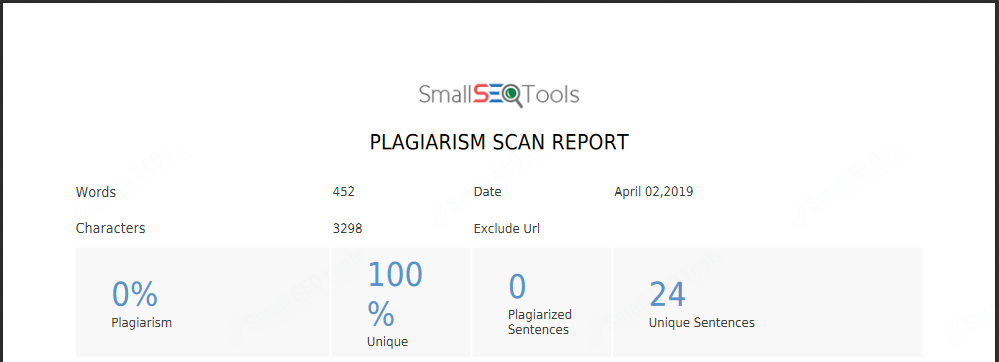
\includegraphics[width=5cm]{figures/5/1174077/teori/plagarismechap5.png}
    \centering
\end{figure}
\end{enumerate}
%%%%%%%%%%%%%%%%%%%%%%%%%%%%%%%%%%%%%%%%%%%%%%%%%%%%%%%%%%%%%%%%%%%%%%%%%%%%%%%%%%%%%%%%%%%%%